% --- LaTeX Lecture Notes Template - S. Venkatraman ---

% --- Set document class and font size ---

\documentclass[letterpaper, 12pt]{article}

% --- Package imports ---

% Extended set of colors
\usepackage[dvipsnames]{xcolor}

\usepackage{
  amsmath, amsthm, amssymb, mathtools, dsfont, units,          % Math typesetting
  graphicx, wrapfig, subfig, float,                            % Figures and graphics formatting
  listings, color, inconsolata, pythonhighlight,               % Code formatting
  fancyhdr, sectsty, hyperref, enumerate, enumitem, framed }   % Headers/footers, section fonts, links, lists

\usepackage{listings}

\lstset{ %
    backgroundcolor=\color{white},   % choose the background color; you must add \usepackage{color} or \usepackage{xcolor}
    basicstyle=\footnotesize\ttfamily,        % the size of the fonts that are used for the code
    breakatwhitespace=false,         % sets if automatic breaks should only happen at whitespace
    breaklines=true,                 % sets automatic line breaking
    captionpos=b,                    % sets the caption-position to bottom
    commentstyle=\color{mygreen},    % comment style
    deletekeywords={...},            % if you want to delete keywords from the given language
    escapeinside={\%*}{*)},          % if you want to add LaTeX within your code
extendedchars=true,              % lets you use non-ASCII characters; for 8-bits encodings only, does not work with UTF-8
frame=single,                    % adds a frame around the code
keepspaces=true,                 % keeps spaces in text, useful for keeping indentation of code (possibly needs columns=flexible)
keywordstyle=\color{blue},       % keyword style
otherkeywords={*,...},            % if you want to add more keywords to the set
numbers=left,                    % where to put the line-numbers; possible values are (none, left, right)
numbersep=5pt,                   % how far the line-numbers are from the code
numberstyle=\tiny\color{mygray}, % the style that is used for the line-numbers
rulecolor=\color{black},         % if not set, the frame-color may be changed on line-breaks within not-black text (e.g. comments (green here))
showspaces=false,                % show spaces everywhere adding particular underscores; it overrides 'showstringspaces'
showstringspaces=false,          % underline spaces within strings only
showtabs=false,                  % show tabs within strings adding particular underscores
stepnumber=2,                    % the step between two line-numbers. If it's 1, each line will be numbered
stringstyle=\color{mymauve},     % string literal style
tabsize=2,                       % sets default tabsize to 2 spaces % show the filename of files included with \lstinputlisting; also try caption instead of title,
}

\renewcommand{\lstlistingname}{Popis}

% lipsum is just for generating placeholder text and can be removed
\usepackage{hyperref, lipsum} 

% --- Fonts ---

\usepackage{newpxtext, newpxmath, inconsolata}

% --- Page layout settings ---

% Set page margins
\usepackage[left=1.35in, right=1.35in, top=1.0in, bottom=.9in, headsep=.2in, footskip=0.35in]{geometry}

% Anchor footnotes to the bottom of the page
\usepackage[bottom]{footmisc}

\usepackage{amsmath, amsfonts, mathtools, amsthm, amssymb}
\usepackage{mathrsfs}

% Set line spacing
\renewcommand{\baselinestretch}{1.2}

% Set spacing between paragraphs
\setlength{\parskip}{1.3mm}

% Allow multi-line equations to break onto the next page
\allowdisplaybreaks

% --- Page formatting settings ---

% Set image captions to be italicized
\usepackage[font={it,footnotesize}]{caption}

% Set link colors for labeled items (blue), citations (red), URLs (orange)
\hypersetup{colorlinks=true, linkcolor=RoyalBlue, citecolor=RedOrange, urlcolor=ForestGreen}

% Set font size for section titles (\large) and subtitles (\normalsize) 
\usepackage{titlesec}
\titleformat{\section}{\large\bfseries}{{\fontsize{19}{19}\selectfont\textreferencemark}\;\; }{0em}{}
\titleformat{\subsection}{\normalsize\bfseries\selectfont}{\thesubsection\;\;\;}{0em}{}

% Enumerated/bulleted lists: make numbers/bullets flush left
%\setlist[enumerate]{wide=2pt, leftmargin=16pt, labelwidth=0pt}
\setlist[itemize]{wide=0pt, leftmargin=16pt, labelwidth=10pt, align=left}

% --- Table of contents settings ---
\usepackage[subfigure]{tocloft}
\usepackage{graphics}
\usepackage{graphicx}

% Reduce spacing between sections in table of contents
\setlength{\cftbeforesecskip}{.9ex}

% Remove indentation for sections
\cftsetindents{section}{0em}{0em}

% Set font size (\large) for table of contents title
\renewcommand{\cfttoctitlefont}{\large\bfseries}

% Remove numbers/bullets from section titles in table of contents
\makeatletter
\renewcommand{\cftsecpresnum}{\begin{lrbox}{\@tempboxa}}
\renewcommand{\cftsecaftersnum}{\end{lrbox}}
\makeatother

\lstdefinelanguage{JavaScript}{
keywords={typeof, new, true, false, catch, function, return, null, catch, switch, var, if, in, while, do, else, case, break},
keywordstyle=\color{blue}\bfseries,
ndkeywords={class, export, boolean, throw, implements, import, this},
ndkeywordstyle=\color{darkgray}\bfseries,
identifierstyle=\color{black},
sensitive=false,
comment=[l]{//},
morecomment=[s]{/*}{*/},
commentstyle=\color{purple}\ttfamily,
stringstyle=\color{red}\ttfamily,
morestring=[b]',
morestring=[b]"
}

\lstdefinelanguage{CSS}{
keywords={accelerator,azimuth,background,background-attachment,
background-color,background-image,background-position,
background-position-x,background-position-y,background-repeat,
behavior,border,border-bottom,border-bottom-color,
border-bottom-style,border-bottom-width,border-collapse,
border-color,border-left,border-left-color,border-left-style,
border-left-width,border-right,border-right-color,
border-right-style,border-right-width,border-spacing,
border-style,border-top,border-top-color,border-top-style,
border-top-width,border-width,bottom,caption-side,clear,
clip,color,content,counter-increment,counter-reset,cue,
cue-after,cue-before,cursor,direction,display,elevation,
empty-cells,filter,float,font,font-family,font-size,
font-size-adjust,font-stretch,font-style,font-variant,
font-weight,height,ime-mode,include-source,
layer-background-color,layer-background-image,layout-flow,
layout-grid,layout-grid-char,layout-grid-char-spacing,
layout-grid-line,layout-grid-mode,layout-grid-type,left,
letter-spacing,line-break,line-height,list-style,
list-style-image,list-style-position,list-style-type,margin,
margin-bottom,margin-left,margin-right,margin-top,
marker-offset,marks,max-height,max-width,min-height,
min-width,-moz-binding,-moz-border-radius,
-moz-border-radius-topleft,-moz-border-radius-topright,
-moz-border-radius-bottomright,-moz-border-radius-bottomleft,
-moz-border-top-colors,-moz-border-right-colors,
-moz-border-bottom-colors,-moz-border-left-colors,-moz-opacity,
-moz-outline,-moz-outline-color,-moz-outline-style,
-moz-outline-width,-moz-user-focus,-moz-user-input,
-moz-user-modify,-moz-user-select,orphans,outline,
outline-color,outline-style,outline-width,overflow,
overflow-X,overflow-Y,padding,padding-bottom,padding-left,
padding-right,padding-top,page,page-break-after,
page-break-before,page-break-inside,pause,pause-after,
pause-before,pitch,pitch-range,play-during,position,quotes,
-replace,richness,right,ruby-align,ruby-overhang,
ruby-position,-set-link-source,size,speak,speak-header,
speak-numeral,speak-punctuation,speech-rate,stress,
scrollbar-arrow-color,scrollbar-base-color,
scrollbar-dark-shadow-color,scrollbar-face-color,
scrollbar-highlight-color,scrollbar-shadow-color,
scrollbar-3d-light-color,scrollbar-track-color,table-layout,
text-align,text-align-last,text-decoration,text-indent,
text-justify,text-overflow,text-shadow,text-transform,
text-autospace,text-kashida-space,text-underline-position,top,
unicode-bidi,-use-link-source,vertical-align,visibility,
voice-family,volume,white-space,widows,width,word-break,
word-spacing,word-wrap,writing-mode,z-index,zoom},
sensitive=true,
morecomment=[l]{//},
morecomment=[s]{/*}{*/},
morestring=[b]',
morestring=[b]",
alsoletter={:},
alsodigit={-}
}

% --- Set path for images ---

\graphicspath{{images/}{../images/}}

% --- Math/Statistics commands ---

% Add a reference number to a single line of a multi-line equation
% Usage: "\numberthis\label{labelNameHere}" in an align or gather environment
\newcommand\numberthis{\addtocounter{equation}{1}\tag{\theequation}}

% Shortcut for bold text in math mode, e.g. $\b{X}$
\let\b\mathbf

% Shortcut for bold Greek letters, e.g. $\bg{\beta}$
\let\bg\boldsymbol

% Shortcut for calligraphic script, e.g. %\mc{M}$
\let\mc\mathcal

% \mathscr{(letter here)} is sometimes used to denote vector spaces
\usepackage[mathscr]{euscript}
\usepackage[croatian]{babel}
% Convergence: right arrow with optional text on top
% E.g. $\converge[p]$ for converges in probability
\newcommand{\converge}[1][]{\xrightarrow{#1}}

% Weak convergence: harpoon symbol with optional text on top
% E.g. $\wconverge[n\to\infty]$
\newcommand{\wconverge}[1][]{\stackrel{#1}{\rightharpoonup}}

% Equality: equals sign with optional text on top
% E.g. $X \equals[d] Y$ for equality in distribution
\newcommand{\equals}[1][]{\stackrel{\smash{#1}}{=}}

% Normal distribution: arguments are the mean and variance
% E.g. $\normal{\mu}{\sigma}$
\newcommand{\normal}[2]{\mathcal{N}\left(#1,#2\right)}

% Uniform distribution: arguments are the left and right endpoints
% E.g. $\unif{0}{1}$
\newcommand{\unif}[2]{\text{Uniform}(#1,#2)}

% Independent and identically distributed random variables
% E.g. $ X_1,...,X_n \iid \normal{0}{1}$
\newcommand{\iid}{\stackrel{\smash{\text{iid}}}{\sim}}

% Sequences (this shortcut is mostly to reduce finger strain for small hands)
% E.g. to write $\{A_n\}_{n\geq 1}$, do $\bk{A_n}{n\geq 1}$
\newcommand{\bk}[2]{\{#1\}_{#2}}

% Math mode symbols for common sets and spaces. Example usage: $\R$
\newcommand{\R}{\mathbb{R}}	% Real numbers
\newcommand{\C}{\mathbb{C}}	% Complex numbers
\newcommand{\Q}{\mathbb{Q}}	% Rational numbers
\newcommand{\Z}{\mathbb{Z}}	% Integers
\newcommand{\N}{\mathbb{N}}	% Natural numbers
\newcommand{\F}{\mathcal{F}}	% Calligraphic F for a sigma algebra
\newcommand{\El}{\mathcal{L}}	% Calligraphic L, e.g. for L^p spaces

% Math mode symbols for probability
\newcommand{\pr}{\mathbb{P}}	% Probability measure
\newcommand{\E}{\mathbb{E}}	% Expectation, e.g. $\E(X)$
\newcommand{\var}{\text{Var}}	% Variance, e.g. $\var(X)$
\newcommand{\cov}{\text{Cov}}	% Covariance, e.g. $\cov(X,Y)$
\newcommand{\corr}{\text{Corr}}	% Correlation, e.g. $\corr(X,Y)$
\newcommand{\B}{\mathcal{B}}	% Borel sigma-algebra

% Other miscellaneous symbols
\newcommand{\tth}{\text{th}}	% Non-italicized 'th', e.g. $n^\tth$
\newcommand{\Oh}{\mathcal{O}}	% Big-O notation, e.g. $\O(n)$
\newcommand{\1}{\mathds{1}}	% Indicator function, e.g. $\1_A$

% Additional commands for math mode
\DeclareMathOperator*{\argmax}{argmax}		% Argmax, e.g. $\argmax_{x\in[0,1]} f(x)$
\DeclareMathOperator*{\argmin}{argmin}		% Argmin, e.g. $\argmin_{x\in[0,1]} f(x)$
\DeclareMathOperator*{\spann}{Span}		% Span, e.g. $\spann\{X_1,...,X_n\}$
\DeclareMathOperator*{\bias}{Bias}		% Bias, e.g. $\bias(\hat\theta)$
\DeclareMathOperator*{\ran}{ran}			% Range of an operator, e.g. $\ran(T) 
\DeclareMathOperator*{\dv}{d\!}			% Non-italicized 'with respect to', e.g. $\int f(x) \dv x$
\DeclareMathOperator*{\diag}{diag}		% Diagonal of a matrix, e.g. $\diag(M)$
\DeclareMathOperator*{\trace}{trace}		% Trace of a matrix, e.g. $\trace(M)$
\DeclareMathOperator*{\supp}{supp}		% Support of a function, e.g., $\supp(f)$

% Numbered theorem, lemma, etc. settings - e.g., a definition, lemma, and theorem appearing in that 
% order in Lecture 2 will be numbered Definition 2.1, Lemma 2.2, Theorem 2.3. 
% Example usage: \begin{theorem}[Name of theorem] Theorem statement \end{theorem}
\theoremstyle{definition}
\newtheorem{theorem}{Theorem}[section]
\newtheorem{proposition}[theorem]{Proposition}
\newtheorem{lemma}[theorem]{Lemma}
\newtheorem{corollary}[theorem]{Corollary}
\newtheorem{definition}[theorem]{Definicija}
\newtheorem{example}[theorem]{Example}
\newtheorem{remark}[theorem]{Remark}


% Un-numbered theorem, lemma, etc. settings
% Example usage: \begin{lemma*}[Name of lemma] Lemma statement \end{lemma*}
\newtheorem*{theorem*}{Theorem}
\newtheorem*{proposition*}{Proposition}
\newtheorem*{lemma*}{Lemma}
\newtheorem*{corollary*}{Corollary}
\newtheorem*{definition*}{Definition}
\newtheorem*{example*}{Example}
\newtheorem*{remark*}{Remark}
\newtheorem*{claim}{Claim}


%
%\declaretheorem[numbered=no, style=thmexplanationbox, name=Proof]{explanation}
%\declaretheorem[numbered=no, style=thmproofbox, name=Proof]{replacementproof}
%\declaretheorem[style=thmbluebox,  numbered=no, name=Exercise]{ex}
%\declaretheorem[style=thmbluebox,  numbered=no, name=Example]{eg}
%\declaretheorem[style=thmblueline, numbered=no, name=Remark]{remark}
%\declaretheorem[style=thmblueline, numbered=no, name=Note]{note}
%
%\renewenvironment{proof}[1][\proofname]{\begin{replacementproof}}{\end{replacementproof}}
%
%\AtEndEnvironment{eg}{\null\hfill$\diamond$}%
%
%\newtheorem*{uovt}{UOVT}
%\newtheorem*{notation}{Notation}
%\newtheorem*{previouslyseen}{As previously seen}
%\newtheorem*{problem}{Problem}
%\newtheorem*{observe}{Observe}
%\newtheorem*{property}{Property}
%\newtheorem*{intuition}{Intuition}
%
%
%\usepackage{etoolbox}
%\AtEndEnvironment{vb}{\null\hfill$\diamond$}%
%\AtEndEnvironment{intermezzo}{\null\hfill$\diamond$}%

% --- Left/right header text (to appear on every page) ---

% Do not include a line under header or above footer
\pagestyle{fancy}
\renewcommand{\footrulewidth}{0pt}
\renewcommand{\headrulewidth}{0pt}

% Right header text: Lecture number and title
\renewcommand{\sectionmark}[1]{\markright{#1} }
\fancyhead[R]{\small\textit{\nouppercase{\rightmark}}}

% Left header text: Short course title, hyperlinked to table of contents
\fancyhead[L]{\hyperref[sec:contents]{\small Uvod u mreže}}

% --- Document starts here ---

\begin{document}

% --- Main title and subtitle ---

\title{\Large{\textbf{\MakeUppercase{Osnove web programiranja}}} \\[1em]
\normalsize \textbf{Uvod u Internet i računalne mreže}}

% --- Author and date of last update ---

\author{\normalsize Karlo Vizec}
\date{\normalsize\vspace{-1ex} Zadnji put ažurirano: \today}

% --- Add title and table of contents ---

\maketitle
\tableofcontents\label{sec:contents}

% --- Main content: import lectures as subfiles ---

% TeX root = ../main.tex


% First argument to \section is the title that will go in the table of contents. Second argument is the title that will be printed on the page.
\section[Računalne mreže]{Računalne mreže}

U početku su računala bila ogromni strojevi, zuzimali su cijele sobe i bili su sporiji od najsporijeg pametnog mobitela.
I što je najbitnije, nisu bila povezana.
Jedno računalo je bilo samo za sebe, nije imalo pristup ostalima, a to je znatno ograničavalo njihovu funkcinonalnost.
Podaci su morali biti prebacivani između računala pomoću fizičkih uređaja, diskete, a to je potrajalo i nije bilo praktično za velike udaljenosti.

Informatičari su to ubrzo shvatili te nije prošlo mnogo vremena od razvoja prvih računala do razvoja prve veće računalne mreže.
Ta je mreža bila \textbf{ARPANET}.
Razvila ju je američka agencija ARPA, sada zvana DARPA, 1969.
Do 1971.\ je imala 15 računala povezana na nju.
Za razliku od današnjeg Interneta, ARPANET bio je znatno manje sofisticiran, sigurnosne mjere nisu postojale, umreženi računala bilo je malo i bio je spor.
Ključna razlika je činjenica da su ARPANET i slične mreže koristili većinom informatički stručnjaci, sveučilišta i vlada, a ne i svakodnevni građani.

Međutim, ARPANET je bio ključan korak u razvoju modernog Interneta.
ARPANET je bio rani primjer većeg \textbf{distribuiranog sustava}.
Distribuirani sustavi su ključni sastojak modernog računarstva jer omogoćuju podjelu rada na više računala, a to znatno povećava performanse.
Jedno računalo, makar bilo i superračunalo, nije dovoljno snažno za zadatke koji zahtjevaju veliku količinu računalnih resursa.
Očiti primjeri su znanstveni izračuni, npr.\ simulacija proteina.
Naravno, sam Internet je najveći primjer masovnog distribuiranog sustava.

\definition{Distribuirani sustav je sustav računalne mreže u koju su povezana dva ili više zasebna računala koja koriste svoje računalne resure za izvršavanje zajedničkog zadatka ili cilja.}

Danas je sve više i više uređaja umreženo.
Štoviše, svjetska ekonomija ovisi o Internetu.
Tijekom zadnjih nekoliko godina, sve je više i Internet of Things (IoT) uređaja, npr. pametni televizori, frižideri, termostati i slično.

\subsection{Osnove vrste i svrha mreža}

Internet kao koncept najlakše se može zamisliti kao \("\)mreža od mreža\("\).
Računalne mreže postoje kako bi omogućile međusobno povezivanje računala i drugih uređaja u svrhe međusobne komunikacije.

Te računalne mreže od kojih se sastoji Internet uključuju one najmanje, \textbf{LAN} (engl. \textit{Local Area Network}) mreže koje se nalaze u kućama i stanovima svih ljudi.

\definition{LAN je vrsta lokalne mreže koja povezuje uređaje na lokalnom prostoru, npr. kućanstvo, sveučilište ili tvrtka.}

One se obično sastoje od rutera, nekoliko računala i mobitela, televizora te još neke opreme.
Sljedeća najbitnija razina mreže je \textbf{WAN} (engl. \textit{Wide Area Network}).
Glavna razlika između WAN i LAN mreža je u geografskom području koje zauzimaju.
WAN mreže će obično imati naprednije sustave koji su potrebni za upravljanje tako velikim prostorom.

\definition{WAN je vrsta mreže koja se sastoji od velikog broja uređaja, najčešće i druge LAN mreže, s velikim opsegom, npr. grad ili država.}

Još kategorija računalnih mreža postoje, uključujući \textbf{Personal Area Network (PAN)} i \textbf{Metropolitan Area Network (MAN)}.
PAN mreže su nekoliko metara u veličini.
Primjer takve mreže su mobitel i slušalice spojene pomoću WiFi-a ili Bluetootha.
MAN mreže obično su one mreže koje povezuju veće područje, recimo neki grad ili naselje.

Pristup Internetu daju pružatelji internetskih usluga (engl. \textit{Internet Service Provider}, \textbf{ISP}).
Primjeri ISP-ova u Hrvatskoj su Hrvatski Telekom, Optima Telekom, A1 i drugi.

\definition{ISP je organizacija (u većini slučajeva komercijalna tvrtka) koja pruža internetske usluge drugim osobama i organizacijama.}

\subsection{Komponente mreža}

Za veliku većinu osoba, pristup Internetu dobiti će u obliku uređaja koji se zove \textbf{ruter} (od engl. \textit{router}).
Ruter je uređaj koji služi kao glavna pristupna točka Internetu, na njega se, žično ili bežično, povezuju drugi uređaji koji zahtjevaju pristup Internetu, ali i ostalim uređajima u LAN mreži.
Njegova svrha je komunikacija između uređaja u njegovoj mreži i šireg Interneta.
On odašilje i prima (te onda šalje uređaju koji je namijenjeni primatelj) pakete podataka koje šalju i primaju uređaji povezani u mrežu putem rutera.

\definition{Ruter je uređaj koji povezuje računalne mreže te računala u njima tako što koordinirate slanje i primanje paketa podataka. Najčešće povezuje lokalnu mrežu s Internetom.}

\begin{figure}[H]\label{fig:lan-diagram}
\centering
\vspace*{-1cm}

\includegraphics[scale=0.1]{lan-diagram}
\vspace*{-1cm}
\caption{Dijagram jednostavne LAN mreže s ruterom i nekoliko uređaja povezanih na njega. Kompliciranije LAN mreže mogu imati i mrežni preklopnik (engl. \textit{switch}). Izvor: Cloudflare.}
\end{figure}

Komponente mreže prikazane na Slici 1.1 jesu one najčešće.
Međutim, postoje i druge komponente mreža.
Ruter, recimo, nije nužan da bi se stvorila mreža.
Primjer uređaja koji može zamjeniti neke svrhe rutera je \textbf{mrežni preklopnik}.
On povezuje računala u mrežu u obliku zvijezde tako što koordinira slanje poruka između računala i omogućava im da komuniciraju međusobno.
Glavna razlika između preklopnika i rutera je ta što preklopnik ne može sam povezati svoju mrežu s vanjskim svijetom Interneta.
Međutim, preklopnici su često spojeni na ruter te tako mogu povezati računala s ostatkom Interneta.

\definition{Mrežni preklopnik je uređaj koji povezuje računala unutar mreže tako što šalje podatkovne pakete na njihovo odredište.}

\begin{figure}[H]\label{fig:switch-lan-diagram}

\includegraphics[scale=0.3,left]{switch-diagram}
\raggedleft
\caption{Dijagram LAN mreže s mrežnim preklopnikom. Izvor: Cloudflare.}
\end{figure}
% TeX root = ../main.tex

\section[Internet]{Internet}

Predače Interneta kao što su ARPANET bile su u početku eksluzivne.
Broj korisnika bio je malen, ograničen na profesijonalne korisnike, uglavnom sveučilišta i vladine organizacije.
Stoga je i broj \textbf{čvorova} bio relativno mali.

Za razliku od ARPANET-a, na Internet su povezane milijarde uređaja, od osobnih računala, servera do pametnih automobila.
Očekuje da će broj ne-IoT uređaja povezanih na Internet (računala, serveri, itd.) u 2025.\ dostići 10 milijardi.
Sam broj uređaja je ogroman, veći je od populacije Zemlje, a svakom godinom se drastično povećava.

\definition{Čvor je fizičko računalo koje je član računalne mreže.}

\begin{figure}[h]\label{fig:arpanet}
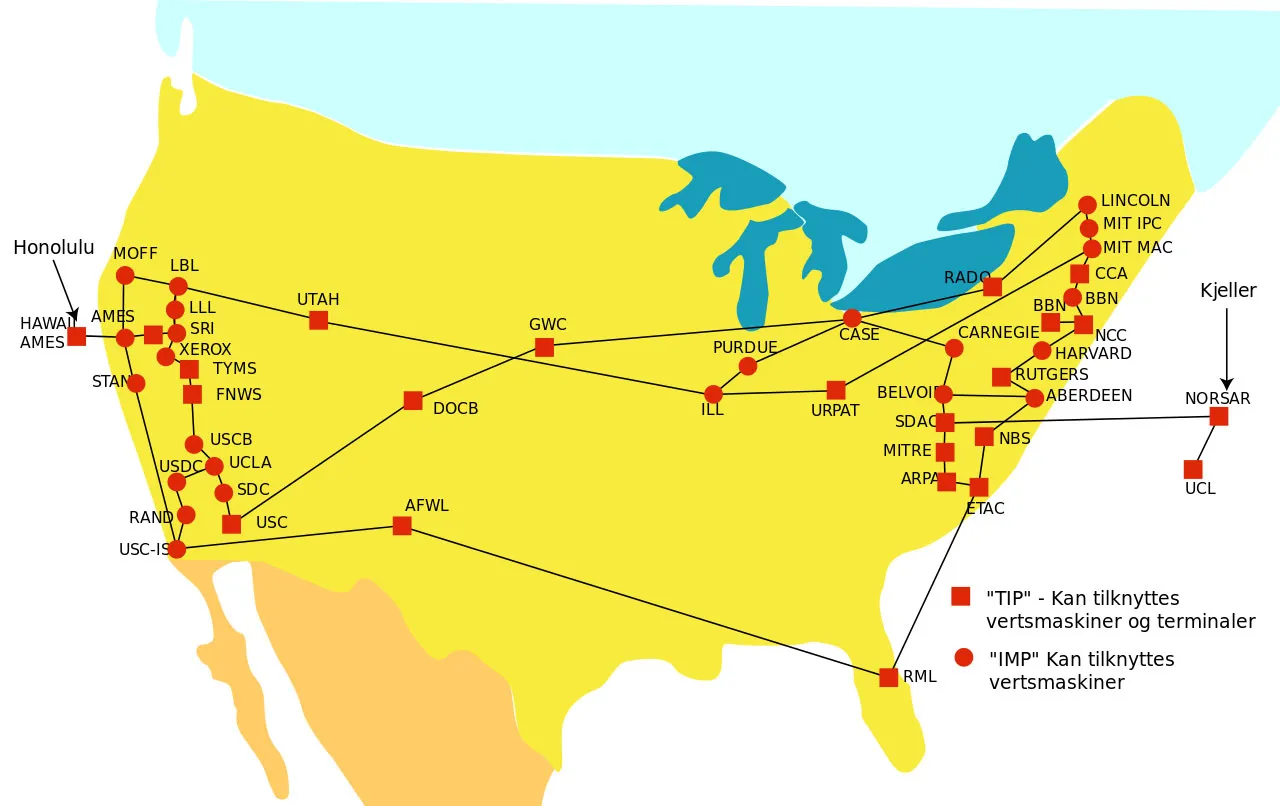
\includegraphics[scale=0.3125,left]{arpanet}
\raggedleft
\caption{Dijagram ARPANET mreže u rujnu 1974. Izvor: Britannica.}
\end{figure}

Dakle, zbog tolikog broja korisnika koje mora služiti, Internet mora biti dizajniran da podrži toliki broj korisnika.
Kao što smo prije spomenuli, Internet je masovni, distribuiran sustav.
Najlakše ga je zamisliti kao \textit{mrežu mreža}: ogromna mreža stvorena od velikog broja manjih mreža, npr. WAN, koje su same stvorene od još manjih mreža, npr. LAN.
Prostire se cijelom Zemljom, prolazi kroz stotine države i svih sedam kontinenata.

Internet načelno nema središnju organizaciju koja njime upravlja.
Malo je čudo što je moguće (na relativno lagan način) napraviti web stranicu kojoj netko može pristupiti putem Interneta iz (više-manje) bilo koje zemlje svijeta na gotovo bilo kojem uređaju s pristupom Internetu.
To je moguće zbog standardizacije koju provede međunarodne organizacije.

Jezgra Interneta sastoji se od nekoliko ogromnih, medunarodnih korporacija (ISP-ova) koji se vlasnici nekoliko skupina međusobno povezanih  mreža s velikim protokom.
Glavni dio tih mreža je skupina podvodnih komunikacijskih kablova koji povezuju Internet izmedu kontinenata.
Te mreže su \textbf{kralježnica Interneta}.
Ti su kablovi bitni geostrateški resursi za države, ali i korporacije.
Pomoću njih obavještajne agencije mogu provoditi kibernetičku špijunažu.\footnote{U SAD-u je ta agencija NSA, a u UK-u GCHQ.}

\begin{figure}[h]
    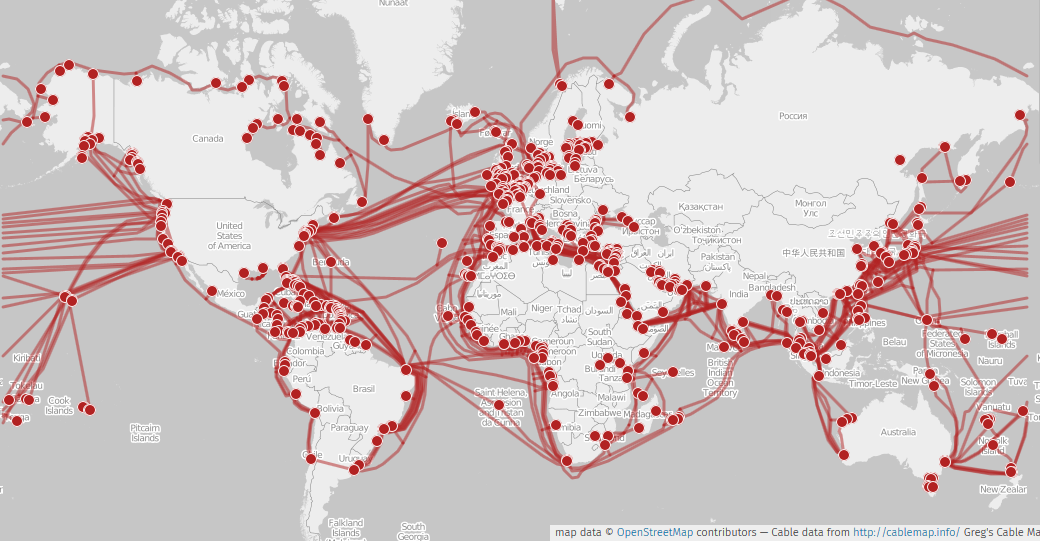
\includegraphics[scale = 0.42]{internet-underwater-backbone}
    \caption{Međukontinentalna mreža podvodnih komunikacijskih kablova koji služe kao kralježnica Interneta iz 2015. Izvor: OpenStreetMap. }\label{fig:figure6}
\end{figure}

\subsection{Adresiranje, domene i DNS}

Svaka web stranica ima svoju adresu.
To je uvjetovano činjenicom da mora postojati neki standardizirani sustav pomoću kojeg će računala pronalaziti jedni druge.
Kroz korištenje Interneta, primjetili ste da koju god stranicu otvorite, vaš preglednik će prikazati neku adresu, npr. \verb|google.com|, \verb|carnet.hr| ili \verb|github.com|.
Takva vrsta web adrese je \textbf{domena}.

\definition{Domena je naziv koji označava određenu web stranicu ili područje unutar Interneta.}

Postoji nekoliko vrsta domena.
Najviša razina su \textbf{vršne domene} (engl. \textit{top-level domains}, \textbf{TLDs}).
One uključuju \verb|.com|, \verb|.net|, \verb|.org|, \verb|.edu|, \verb|.hr|.

Vršne domene se mogu nadalje podjeliti na \textbf{generičke domene} (\textbf{gTLDs}, npr. \verb|.com|, \verb|.edu|, \verb|.net|, itd.) i \textbf{geografske domene} (\textbf{ccTLDs}, npr. \verb|.hr|, \verb|.us|, \verb|.uk|, \verb|.de|, itd.).
Generičke domene sastoje se od tri znaka, a geografske od dva.
Pomoću vršnih domena mogu se registrairati vlastite domene preko \textbf{registara domena}.

\definition{Registar domena je organizacija koja je dobila dozvolu od ICANN-a da korisnicima nudi (većinom komercijalnu) uslugu registracije, odnosno kupnje, domena.}

Gotovo svaka stranica na Webu ima svoju domenu.
Domene nisu ni skupe za registrirati.
Prosječna \verb|.com| ili \verb|.net| domena košta oko 10€ godišnje.
Uz domene je moguće registrirati i beskonačni broj \textbf{poddomena}, npr. \verb|ocjene.skole.hr| ili \verb|www.google.com|.
Organizacija koja je zadužena za upravljanjem domena je Internetska korporacija za dodjeljena imena i brojeve (engl. \textit{Internet Corporation for Assigned Names and Numbers}, \textbf{ICANN}).

Međutim, iako su domene korisne za lako pamćenje i navigiranje Internetom, one nisu zapravo način na koji su uređaji na Internetu adresirani.
Iza svake domene leži IP (engl. \textit{Internet Protocol}) adresa.
IP je mrežni protokol (O mrežnim protokolima ćemo detaljnije u sljedećem poglavlju.) koji omogućava da uređaji u mreži međusobno šalju informacije.
Ta mreža ne mora biti Internet.
U IP-u, podaci se šalju u obliku \textbf{podatkovnih paketa}.
Svaki podatkovni paket sadrži metapodatke, adresu pošiljatelja, primatelja, i slično, te sam sadržaj paketa.

Svaki uređaj povezan u bilo koju vrstu računalne mreže, npr.\ preko rutera, dobiti će svoju jedinstvenu, lokalnu IP adresu.
Naravno, svaki uređaj također ima i javnu IP adresu, onu vidljivu uređajima na širem Internetu.
Važno je naglasiti da (u kućnim LAN mrežama) javnu IP adresu obično nema svaki pojedini uređaj; ruter ima svoju javnu IP adresu koja je onda zajednička svim uređajima koji su povezani pomoću njega.\footnote{Za veliku većinu nekomercijalnih korisnika Interneta, njihova javna IP adresa je dinamička, što znači da se svako malo mjenja. Statičke IP adrese se obično koriste kada je računalo ujedno i server.}

IP adrese su brojevi.
Najčešći oblik IP adrese su \textbf{IPv4 adrese}\footnote{IPv4 označuje četvrtu verziju Internet Protokola.}.
IPv4 adrese sastoje se od 32 bita, što znači da je maksimalni broj IPv4 adresa $ 2^{32} $ (4,294,967,796).
Drugim riječima, najveći broj uređaja koji mogu biti adresirani na Internetu pomoću IPv4 adresa je $ 2^{32} $.

IPv4 adrese se zapisuju u obliku četiri 8-bitnih brojeva odjeljeni s točkom: \verb|A.B.C.D|.
Primjeri IPv4 adresa uključuju \verb|8.8.8.8|, \verb|245.40.3.36| i \verb|127.0.0.1|.
IP adresa \verb|127.0.0.1| je rezervirana te označava računalo koje je poslalo zahtjev, njezina kratica je \verb|localhost|.
Drugim riječma, bilo koji promet poslan na nju biti će vraćen nazad pošiljatelju.
Najveći osmobitni broj je $ 2^8 - 1 $ (255).
Dakle, svaki broj u IPv4 adresi ne može biti veći od 255, odnosno najveća IPv4 adresa je \verb|255.255.255.255|.

U početku je to bilo više nego dovoljno.
Nitko nije mogao predvidjeti da će Internet postati ovako veliki kakva je danas.
Polako je to postalo nedovoljno jer se sve više računala povezivalo na Internet.
IPv4 adrese postaju sve skuplje zbog toga (velika potražnja, mala ponuda).
Internet je danas u procesu prebacivanja na \textbf{IPv6 adrese} koje se sastoje od 128 bitova.
Dakle, s IPv6 adresama, je moguće adresirati $ 2^{128} $ uređaja na Internetu.
IPv6 adrese se zapisuju u obliku osam četveroznamenkastih heksadekadskih brojeva odvojeni s dvotočkom, npr. \verb|6802:f535:52bb:a290:a069:5e2e:470c:c3ca|.

Prevođenje između domena, jezik koji ljudi koriste za pronalazak stranica, i IP adresa, jezik koji koriste računala, događa se preko DNS-a (engl. \textit{Domain Name System}).
DNS sustav sastoji se od \textbf{imenskih servera} koji zapravo provode prevođenje između domena i IP adresa.
Također, DNS je hijerarhiski.
To znači da ne mora svaki imenski server sadržavati popis svih domena i pripadajućih IP adresa već samo mali komad.
Kada preglednik otvara neku stranicu, zatražiti će od DNS-a da prevede tu domenu u IP adresu.
DNS će prvo provjeriti lokalni spremnik, ako tamo nema zapisa ili ako IP adresa više nije valjana, onda će zahtjev prosljediti mjerodavnijem imenskom serveru, npr.\ od ISP-a, sve dok ne dođe to točne IP adrese koju će onda vratiti pregledniku.

\definition{Imenski server je server u DNS-u koji procesira zahtjeve za prevođenje (rezoluciju) domena u IP adrese.}

\begin{figure}[h]
    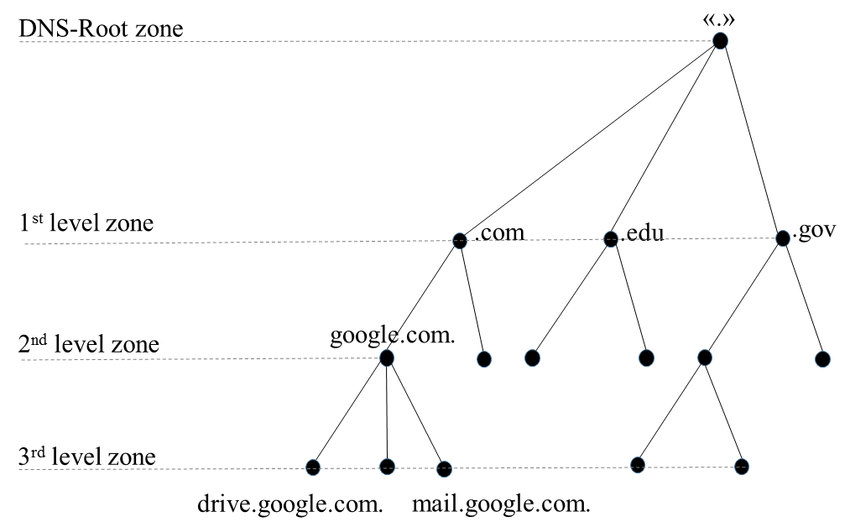
\includegraphics[scale = 0.5]{dns}
    \caption{Hijerarhija DNS-a.}\label{fig:dns}
\end{figure}

\subsection{Mrežni protokoli}

Svaki računalni sustav ima u sebe ugrađene protokole.
Oni mogu biti implicitni, programer može napraviti protokol bez da to primjeti.
Uzmimo za primjer aplikaciju kao što je WhatsApp.
Ona mora obavijestiti korisnika kada je primio nove poruke.
Jednostavna verzija protokola za provjeru dostupnosti novih poruka može biti sljedeća:
\begin{enumerate}
    \item Klijent (aplikacija) šalje zahtjev serveru za provjeru novih poruka.
    \item Server provjeri s bazom podataka jesu li dostupne nove poruke.
    \item Server odgovori klijentu: (a) ako su nove poruke dostupne, odgovori da su dostupne i pošalje nazad te poruke ili (b) ako nisu dostupne, odgovori da nema novih poruka.
    \item Klijent obavijesti server da je primio poruke.
    \item Server označi u bazi podataka da su te poruke poslane klijentu, odnosno da više nisu nove.
    \item Klijent i server zatvore vezu.
    \item Klijent pričeka 15 sekundi prije no što ponovi zahtjev za provjeru.
\end{enumerate}

Ovakav protokol bi radio, ali nije najbolje rješenje.
Glavne mane su mu to što:
\begin{enumerate}
    \item Korisnik mora čekati najviše 15 sekundi prije nego što može primiti poruku. Kod suvremenih aplikacija to vrijeme je znatno manje.
    \item Klijent će često naletiti na situaciju gdje šalje nepotrebne zahtjeve serveru kada novih poruka nema te na taj način oduzima dragocjeno vrijeme serveru.
    \item Server neće prekinuti vezu ako klijent nije poslao obavijest da je primio poruku nakon nekog vremena.
    \item Nema mehanizam da server ponovno pokuša poslati poruke klijentu ako u prijašnjem pokušaju nije obavijestio server da je primio poruke.
\end{enumerate}

Bolje rješenje bilo bi ono u kojem server obavještava korisnika kada su nove poruke dostupne, umjesto da klijent svakih nekoliko sekundi ili minuta šalje zahtjev serveru.
Tako bi korisnik vrlo brzo saznao da su mu poslane nove poruke i mreža bi bila pod puno manjim opterećenjem jer se zahtjevi šalju samo kada je to nužno.
Iz ovog primjera možemo izvesti sljedeću definiciju protokola.

\definition{Mrežni protokol je (obično standardizirani) skup pravila koja omogućuju koordinaciju i komunikaciju između dva ili više programa ili računala u mreži.}

Nakon IP-a, sljedeći najbitniji protokol koji tvori TCP/IP skup protokola je \textbf{TCP} (engl. \textit{Transmission Control Protocol}).
U prijašnjem poglavlju smo rekli da IP omogućuje uređajima da međusobno šalju podatke u obliku podatkovnih paketa.
Međutim, tu IP staje.
IP se bavi isključivo slanjem informacije između računala, a ne i među programima unutar tih računala.
Za to nam treba TCP.
Svaki program koji ima otvorenu vezu prema nekom drugom računalu ili programu imati će dodjeljeni \textbf{port}.

\definition{Port je broj veličine 16 bitova koji omogućuje TCP-u da unutar jednog računala ispravno i precizno šalje podatkovne pakete na njihova odredišta.}

Kako je port broj od 16 bitova, najveći port je \verb|65535|.
Port se zapisuje nakon IP adrese i od nje odvaja dvotočkom, npr. \verb|127.0.0.1:443|.

\begin{table}[]
    \begin{tabular}{|l|l|l|}
        \hline
        \multicolumn{1}{|c|}{\textbf{Rezervirani port}} & \multicolumn{1}{c|}{\textbf{Protokol}} & \textbf{Svrha protokola}                                                                                                     \\ \hline
        21                                              & FTP                                    & Slanje i primanje datoteka i mapa između računala.                                                                           \\ \hline
        80                                              & HTTP                                   & Glavni protokol za web stranice i web servere.                                                                               \\ \hline
        443                                             & HTTPS                                  & \begin{tabular}[c]{@{}l@{}}Sigurna verzija HTTP-a koja osigurava da samo\\ klijent i server mogu čitati poruke.\end{tabular} \\ \hline
        22                                              & SSH                                    & Sigurno povezivanje na terminal servera.                                                                                             \\ \hline
        25                                              & SMTP                                   & Slanje i primanje elektroničke pošte.                                                                                        \\ \hline
        53                                              & DNS                                    & Prevođenje domena u IP adrese.                                                                                               \\ \hline
    \end{tabular}
    \centering
    \caption{Popis čestih rezerviranih portova i pripadajućih protokola.}
    \label{tab:ports}
\end{table}


% TeX root = ../main.tex

\section[World Wide Web]{World Wide Web}

World Wide Web je stvorio znanstvenik u CERN-u Tim Berners-Lee.
CERN je mjesto gdje fizičari bombardiraju čestice s drugim česticama u nadi da će otkriti kako radi svemir.
Međutim, Berners-Lee, koji je bio manje zainteresiran za uništavanje svijeta od ostalih, je vidio problem u trenutnom načinu djeljenja informacija između znanstvenicima.
On je predložio ideju hiperteksta.
Hipertekst je tekst koji u sebi ima poveznice na druge povezane tekstove.
Vidio je priliku da se taj koncept napravi pomoću TCP/IP-a.
Godine 1990.\ je napravio prvu verziju \textbf{HTTP-a} (engl. \textit{HyperText Transfer Protocol}).
HTTP je isto aplikacijski protokol.

Ta je ideja vrlo brzo zaživjela i drugi znanstvenici, ali i drugi korisnici, su se ubrzo pridružili.
Ubrzo je osnovan World Wide Web Consortium (\textbf{W3C}), neprofitna organizacija s ciljem poboljšanja Weba.
Web i Internet se često poistovjećuju, ali oni nisu ista stvar.
Web je skup aplikacija koji leže na temelju Interneta, kao što vidimo.

\subsection{HTTP i prijatelji}

\subsubsection{TLS/SSL}

Suvremeni HTTP je znatno drugačiji od originalne verzije.
Kao i SMTP, bio je napravljen u doba kada računalna sigurnost nije bila u prvom planu jer je vrlo malo ljudi zapravo koristili računala.
Pa tako nije imao ugrađenu podršku za enkripciju komunikacije između HTTP servera i preglednika.
Ta je mana ubrzo uočena kada je Web postajao sve popularniji.
Tvrtka Netscape, koja je tada proizvodila poznati web preglednik Netscape Navigator, razvila je prvu verziju protokola za sigurnu komunikaciju pomoću HTTP-a, \textbf{SSL} (engl. \textit{Secure Sockets Layer}).
SSL je uklopljen u HTTP kao unaprijeđeni protokol \textbf{HTTPS}.
Danas je \textbf{TLS} (engl. \textit{Transport Layer Security}) zamjenio SSL\.

\subsubsection{Klijenti i serveri}

HTTP server se često naziva i \textbf{web server}.
HTTP koristi \textbf{HTTP metode} za izvršavanje zahtjeva.
Metoda govori koja vrstu akcije izvršava određeni URL na serveru.
HTTP zahtjev se sastoji od metode, URL-a zahtjeva, tijela (sadržaja) zahtjeva, verzije HTTP-a i \textit{headera} koji sadrže metapodatke o zahtjevu.

\begin{table}[]
    \begin{tabular}{|l|l|}
        \hline
        \textbf{Metoda} & \textbf{Svrha metode}                                                                                                \\ \hline
        GET             & Dobivanje informacija o nekom resursu, npr. korisnicima, od servera. GET zahtjev ne smije imati tijelo.              \\ \hline
        POST            & Stvaranje novog resursa na serveru, npr. novog korisnika. Obično sadrži tijelo, npr. ime, email i lozinka korisnika. \\ \hline
        PUT             & Promjena resursa na serveru, npr. lozinka korisnika, tako što server zamjeni cijeli resurs.                          \\ \hline
        PATCH           & Promjena resursa na serveru tako što server zamjeni samo taj podatak koji se mjenja.                                 \\ \hline
        DELETE          & Brisanje resursa sa servera.                                                                                         \\ \hline
    \end{tabular}
    \caption{Popis najčešćih HTTP metoda i njihovih svrha.}
    \label{table:http-metode}
\end{table}

Svaki HTTP zahtjev mora dobiti i odgovor koji se sastoji od HTTP koda i tijela odgovora.
Tijelo nije obavezno.

\begin{table}[]
    \begin{tabular}{|l|l|}
        \hline
        \textbf{Kod odgovora}     & \textbf{Značenje}                                                              \\ \hline
        200 OK                    & Zahtjev je uspješno izvršen, zatražene informacije su poslane u odgovoru.      \\ \hline
        201 Created               & Zahtjev je uspješno izvršen, novi resurs je stvoren na serveru.                \\ \hline
        307 Temporary Redirect    & Server preusmjeri zahtjev s istom metodu na drugi URL.                         \\ \hline
        400 Bad Request           & Klijent je krivo formatirao zahtjev.                                           \\ \hline
        401 Unauthorized          & Zahtjev nije uspio, klijent se prvo mora autentificirati, odnsono reći tko je. \\ \hline
        403 Forbidden             & Klijent nema dozvolu pristupiti tom resursu.                                   \\ \hline
        404 Not Found             & Zatraženi resurs ne postoji na serveru.                                        \\ \hline
        500 Internal Server Error & Postoji problem na serverskoj strani koja onemogućuje izvršavanje zahtjeva.    \\ \hline
    \end{tabular}
    \caption{Popis najbitnijih kodova HTTP odgovora i njihovih značenja.}
    \label{tab:http-kodovi}
\end{table}

HTTP kodovi 200--299 označuju uspješan zahtjev, 300--399 preusmjeravanje, 400--499 klijentsku pogrešku i 500--599 serversku pogrešku.

Poznati web serveri uključuju Nginx i Apache HTTP Server.
Tijelo HTTP zahtjeva i odgovora može biti bilo koji oblik podataka.
Tip podataka se određuje pomoću \verb|Content-Type| headera.
Kada preglednik otvara neku stranicu, web serveru će poslati \verb|GET| zahtjev na domenu, odnosno IP adresu, te stranice.
Server će vratiti odgovor s kodom \verb|200 OK| ako stranica postoji ili \verb|404 Not Found| ako ne postoji.
Ako postoji, također će vratiti i tijelo sa HTML kodom stranice.

Tijela HTTP zahtjeva koji se šalju nekom API-u obično zapisuju pomoću \textbf{JSON-a} (engl. \textit{JavaScript Object Notation}).
To je format koji je čitljiv računalima i ljudima, a relativno je jednostavan.
Prije se koristio \textbf{XML} (engl. \textit{Extended Markup Langauge}), ali ga je JSON zamjenio jer je jednostavniji i sadrži manje sigurnosnih propusta.

\subsection{Programiranje na Webu}

Kada je Berners-Lee napravio HTTP, želio je napraviti jednostavan jezik za izradu web stranica.
Odlučio je napraviti \textit{markup jezik}.
To je jednostavan jezik, bazirao ga je na SGML jeziku.
Nazvan je \textbf{HTML} (engl. \textit{HyperText Markup Language}).

\lstinputlisting[language=HTML, label={lst:uvod-u-html}, caption={Osnovna struktura HTML dokumenta.}]{kod/uvod-u-html-1/index.html}

Dakle, stranice su na početku bile jednostavne, tekst s poveznicama, nisu ni imale slike.
Kasnije je HTML dobio i sposobnost dodavanja slika, naravno, i drugih vrsta medija.
Međutim, HTML nema mogućnost promjenu stila web stranice, npr.\ boju teksta ili font teksta ili lokaciju elemenata.
Za to je napravljen \textbf{CSS} (engl. \textit{Cascading Style Sheets}).

\lstinputlisting[language=CSS, label={lst:uvod-u-css}, caption={Primjer CSS koda.}]{kod/uvod-u-css-1/style.css}

Ubrzo su programeri željeli i mogućnost dodavanje interaktivnosti web stranicama.
Do tada su web stranice bile statičke: korisnici nisu mogli interaktirati s njima.
\textbf{JavaScript} (JS) je programski jezik koji je napravio Brendan Eich u 10 dana namjenjen da posluži kao jednostavni jezik za skriptiranje na web stranicama.
U početku je to i bio, koristio se isključivo na web stranicama.
Bio je na neki način baziran na Javi jer je tada Java bila vrlo popularna pa je Netscape, tvrtka koja je zaposlila Eicha da napravi JS, želio da bude slična Javi.
S vremenom su se Java i JavaScript krenuli razilaziti.
Dakle, JavaScript nije jednostavnija verzija Jave nego je svoji samostalan jezik.

Od 2009. JS se sve više koristi za programiranje i izradu servera, mobilnih i desktop aplikacija i drugih proizvoda.
To je omogućio Ryan Dahl, koji je 2009. napravio Node.js, izvršno okruženje koje JavaScriptu daje sve biblioteke i sposobnosti koju imaju ostali jezici.
Pod time uglavnom govorimo o pristupu resursima operacijskog sustava, npr. pristup datotekama, mreži, itd.

Godine 2017. je izašao \textbf{WebAssembly} (WASM), međukod koji omogućuje da se gotovo bilo koji programski jezik izvršava na web stranicama.
Većina popularnih programskih jezika imaju barem djelomičnu podršku za WASM.

\lstinputlisting[language=JavaScript, label={lst:uvod-u-js}, caption={Primjer JavaScript koda.}]{kod/uvod-u-js-1/main.js}


% --- Bibliography ---

% Start a bibliography with one item.
% Citation example: "\cite{williams}".

% --- Document ends here ---

\end{document}
